\chapter{Markov Chain Monte Carlo (MCMC)}

\section{Introduction}

In this section, we will discuss a powerful technique called Markov Chain Monte Carlo (MCMC) that is used to sample from the posterior distribution. MCMC is a class of algorithms that are used to sample from a probability distribution. The basic idea behind MCMC is to construct a Markov chain that has the desired distribution as its equilibrium distribution. The chain is then run for a large number of iterations and the samples generated are used to approximate the desired distribution. \\

The main advantage of MCMC is that it allows us to sample from complex, high-dimensional distributions that are difficult to sample from using other methods. MCMC is widely used in Bayesian statistics, machine learning, and other fields where sampling from complex distributions is required. \\

The idea is to compare generated samples with the target distribution and make small changes to the samples in order to make them more closely resemble the target distribution. This process is repeated until the samples are close enough to the target distribution. \\

\section{Markov Chains}

A Markov chain is a stochastic process that moves from one state to another according to a set of transition probabilities. The state of the chain at time $t$ is denoted by $X_t$, and the transition probabilities are denoted by $P(X_{t+1} | X_t)$. A Markov chain is said to be \textit{homogeneous} if the transition probabilities do not depend on time. \\

A Markov chain is defined by its state space, transition probabilities, and initial distribution. The state space is the set of all possible states that the chain can be in, and the transition probabilities specify the probability of moving from one state to another. The initial distribution specifies the probability of starting in each state. \\

A Markov chain is said to be \textit{irreducible} if it is possible to move from any state to any other state with positive probability. A Markov chain is said to be \textit{aperiodic} if the greatest common divisor of the lengths of all cycles in the chain is 1. A Markov chain that is both irreducible and aperiodic is said to be \textit{ergodic}. \\

An ergodic Markov chain has a unique stationary distribution, which is the distribution that the chain converges to as the number of iterations goes to infinity. The stationary distribution is also known as the equilibrium distribution or the limiting distribution. \\

\section{Fitting GW170817 Light Curve Data}

In this section, we will use MCMC to fit the light curve data from the GW170817 event. The light curve data consists of Observed Frequency and the flux density at each time step. We will use MCMC to sample from the posterior distribution of the parameters of the light curve model. \\

Light curves are graphical representations of the variation in brightness or flux of an astronomical object over time. Fitting light curves with models allows us to extract valuable information about the physical processes governing these sources. The smooth broken power-law model is one such model used to describe the flux evolution. \\

The light curve model is given by the following equation:

\begin{equation}
	F(t, \nu) = 2 ^ {\frac{1}{s}} \left(\dfrac{\nu}{3 \text{ GHz}}\right) ^ \beta \left[\left(\dfrac{t}{t_p} \right)^{-s \alpha_1} + \left(\dfrac{t}{t_p} \right)^{-s \alpha_2}\right] ^ {\frac{-1}{s}}
	\label{eq:smooth_broken_power_law}
\end{equation}

where:

\begin{itemize}
	\item $s$ is the spectral index.
	\item $F_p$ is the flux density at $3$ GHz at the light curve peak.
	\item $\beta$ is the spectral index.
	\item $t$ is the time post-merger.
	\item $t_p$ is the lightcurve peak time.
	\item $\alpha_1$ and $\alpha_2$ are the power-law rise and decay slopes respectively.
	\item $F(t, \nu)$ is the flux density at time $t$ and frequency $\nu$.
\end{itemize}

This is the initial Flux Density \textit{vs} Time data:

\begin{figure}[H]
	\centering
	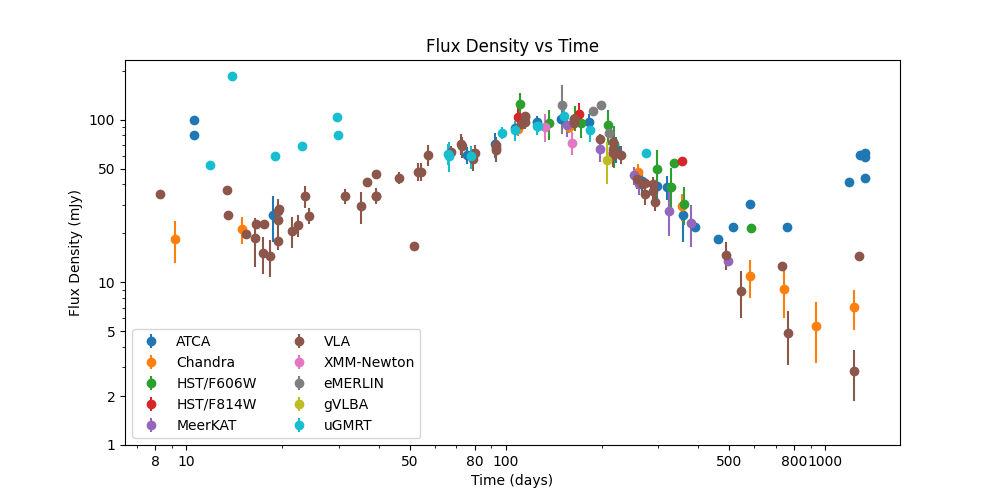
\includegraphics[width=\textwidth]{Images/FluxDensityvsTime.png}
	\caption{Flux Density \textit{vs} Time}
	\label{fig:flux_density_vs_time}
\end{figure}

And this is the corner plot which we get on running the MCMC Algorithm:

\begin{figure}[H]
	\centering
	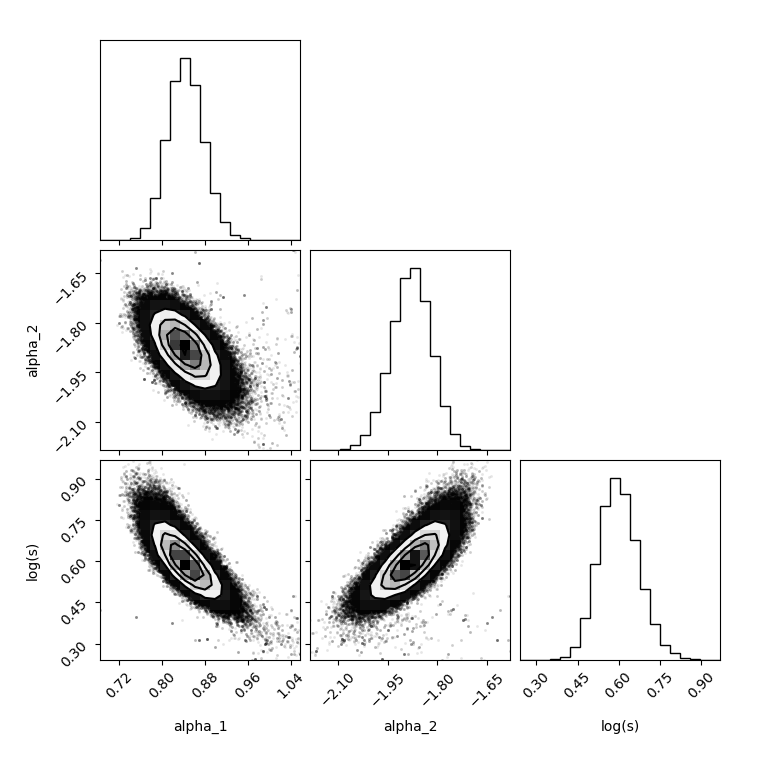
\includegraphics[width=\textwidth]{Images/corner_plot.png}
	\caption{Corner Plot}
	\label{fig:corner_plot}
\end{figure}

\clearpage

Finally this is the best fit light curve model:

\begin{figure}[H]
	\centering
	\includegraphics[width=\textwidth]{Images/Best_fit_model.png}
	\caption{Best Fit Light Curve Model}
	\label{fig:light_curve_model}
\end{figure}

Running MCMC for all parameters raised the \verb|WARNING:root:Too few points to create valid contours|, so I decided to run MCMC for only 3 parameters at a time. The corner plot shows the posterior distribution of the parameters, and the best fit light curve model is shown in the last figure.


